\section{ИССЛЕДОВАНИЕ РАБОТЫ ШИФРАТОРА}

\begin{figure}[H]
	\centering
	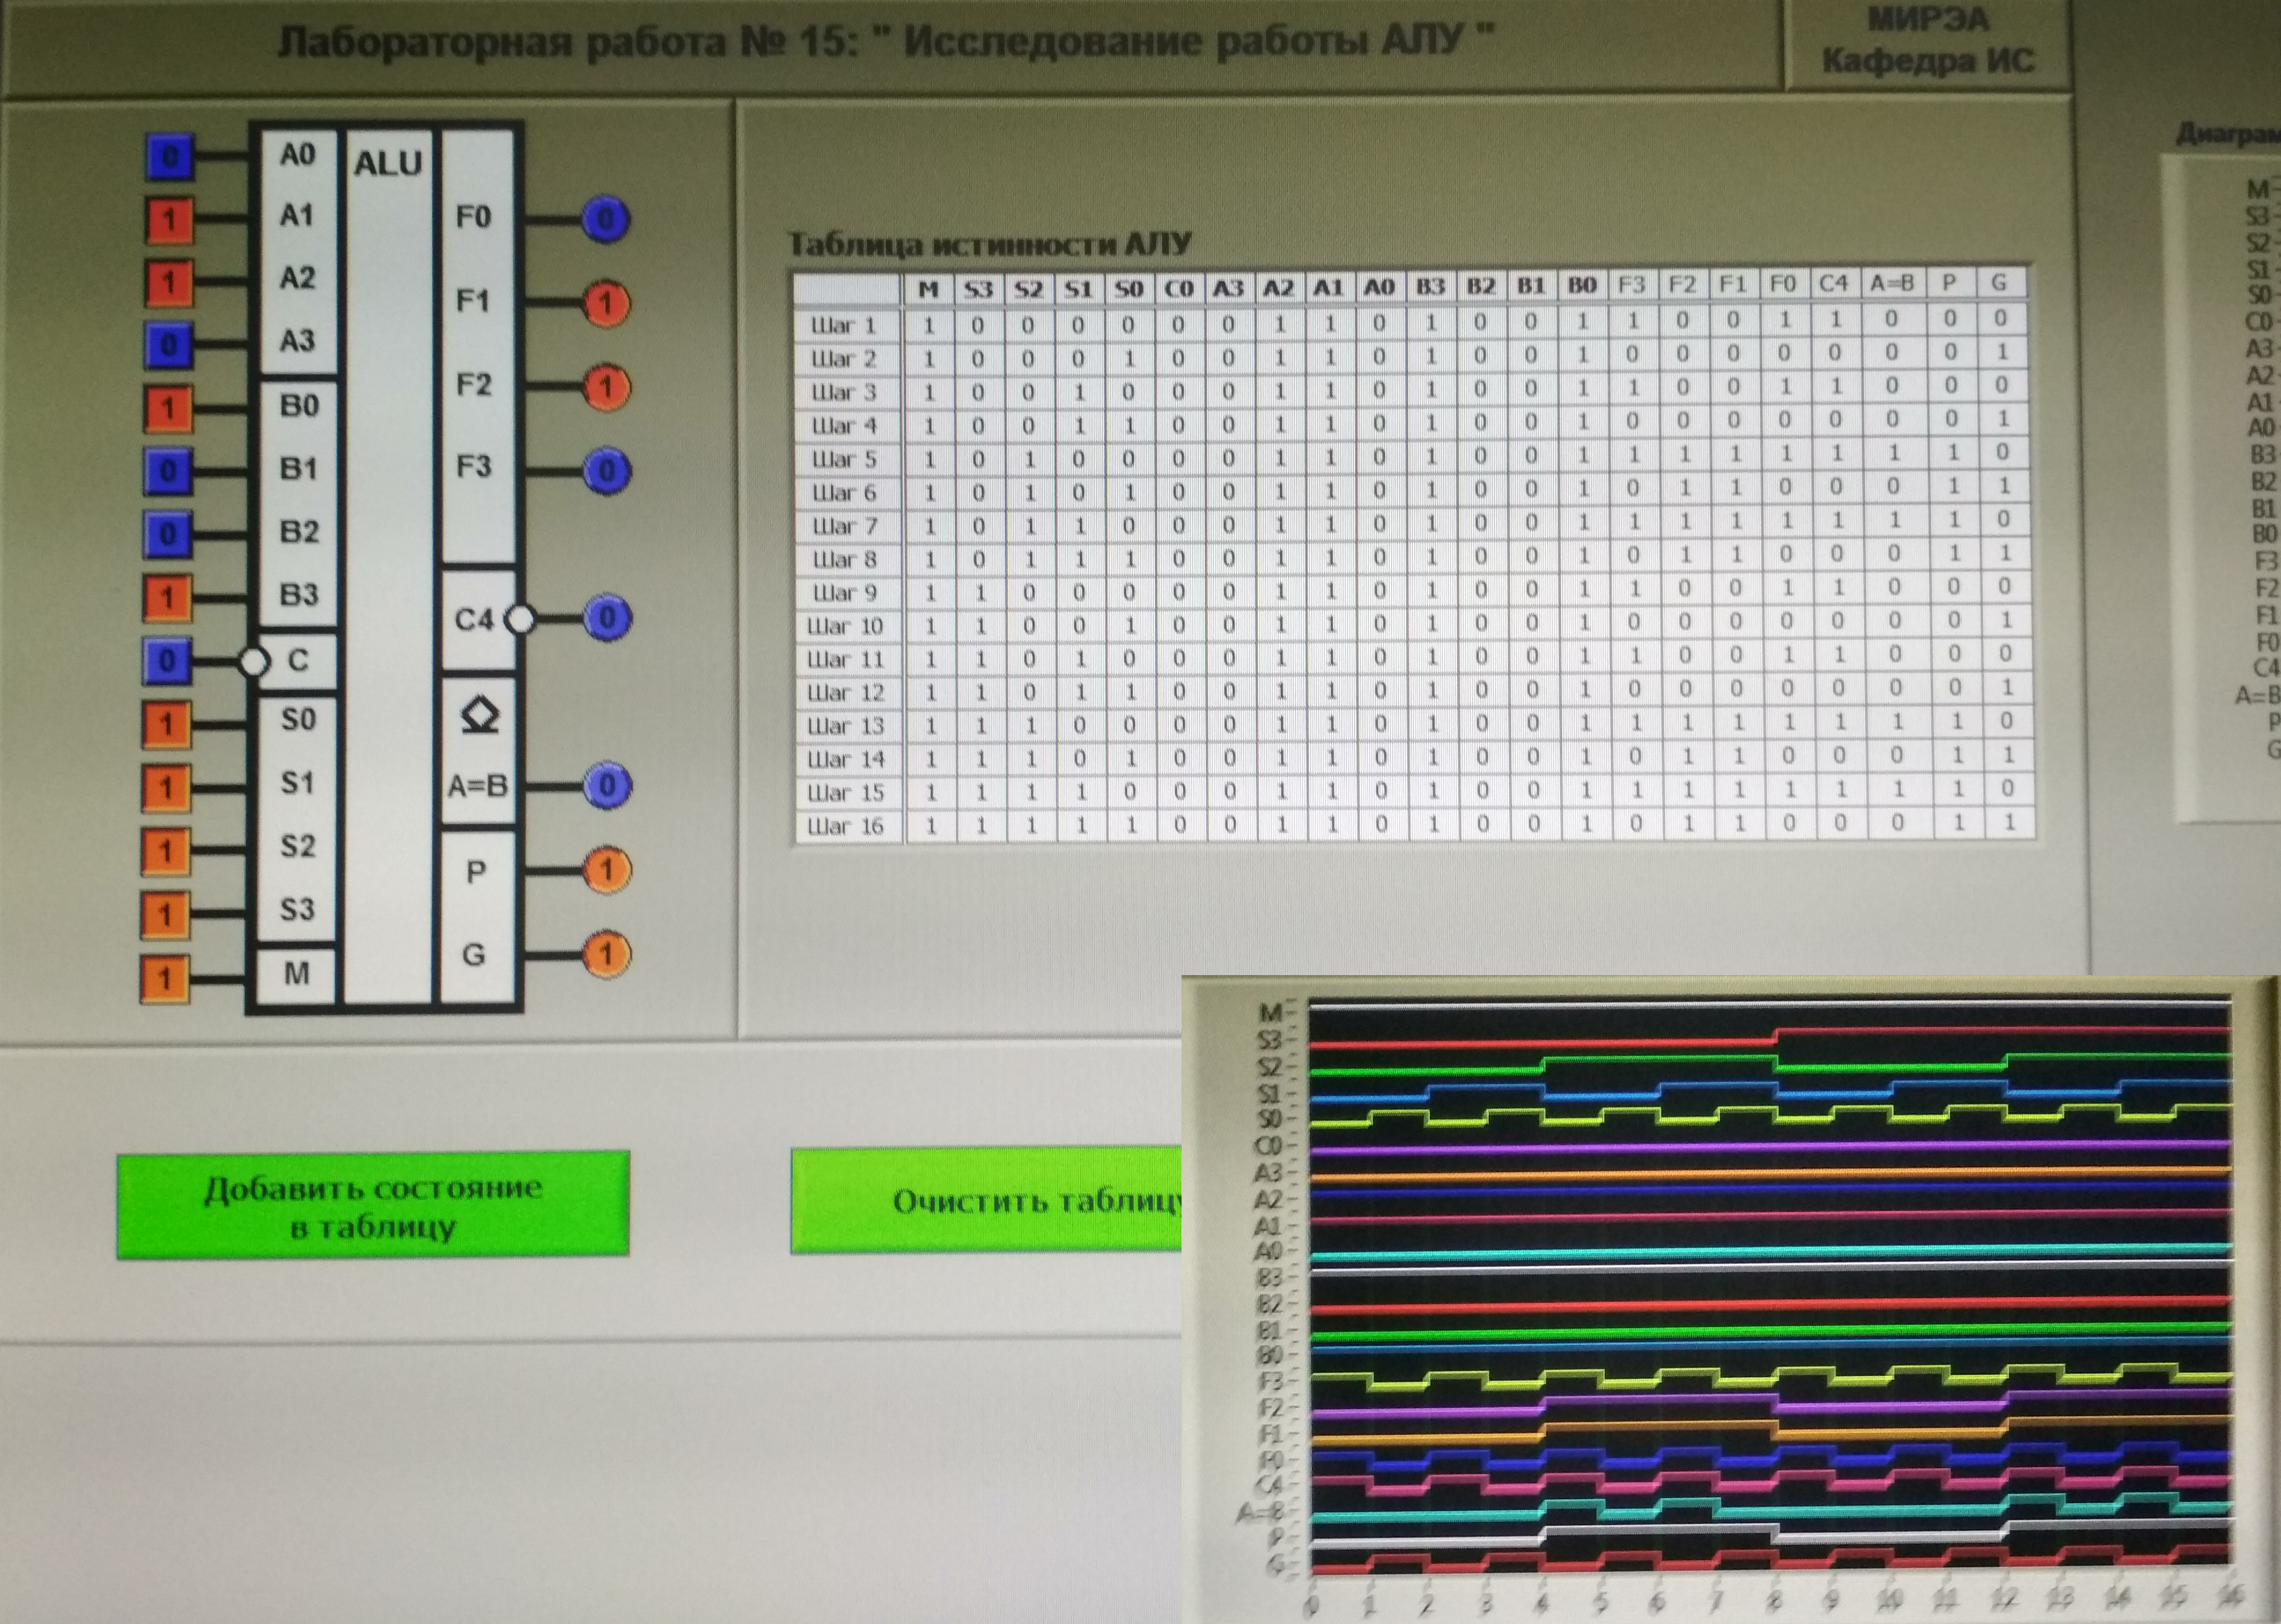
\includegraphics[width=0.95\linewidth]{imgs/2/1}
	\caption{Результат работы включенного шифратора}
	\label{fig:2_on}
\end{figure}

\begin{figure}[H]
	\centering
	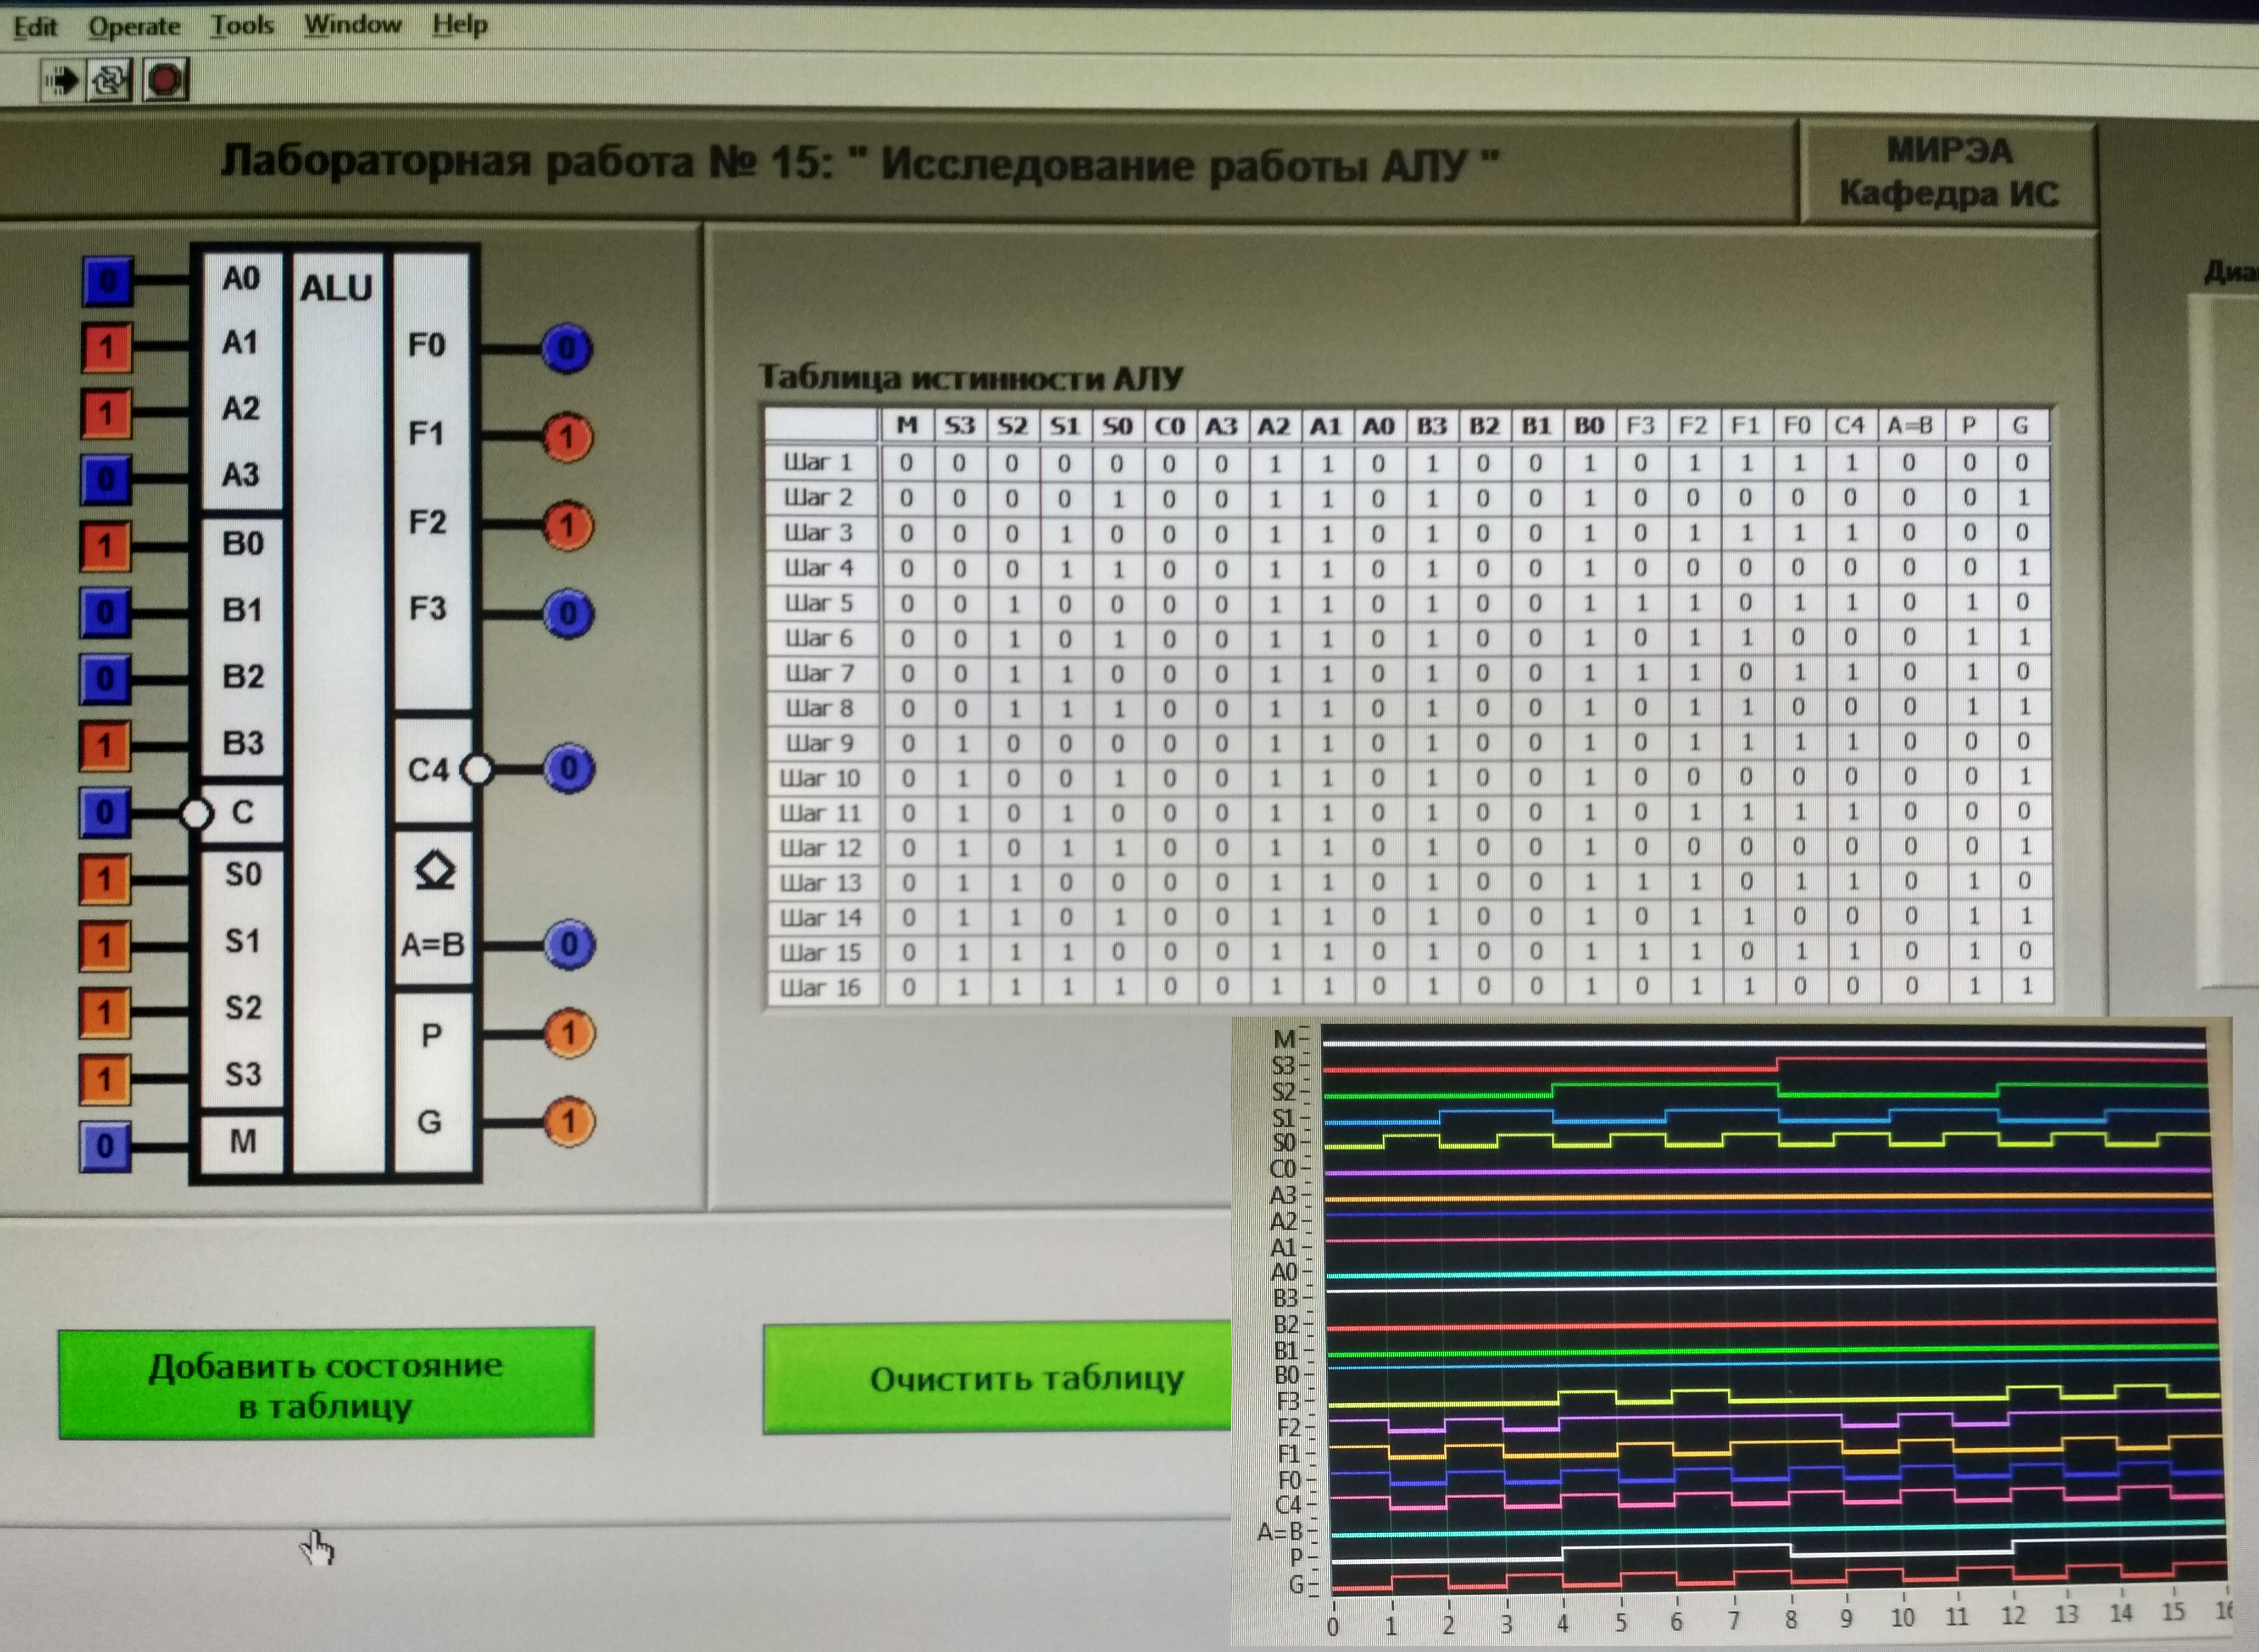
\includegraphics[width=0.95\linewidth]{imgs/2/2}
	\caption{Результат работы выключенного шифратора}
	\label{fig:2_off}
\end{figure}

В ходе работы было выяснено, что для работы шифратора необходимо подать низкий уровень на вход E.
Активный сигнал на выходе G наблюдается при подаче хотя бы одного сигнала.
Выход E0 становится неактивным, если есть хотя бы 1 сигнал.
% Шифратор является приоритетным, вход X6 имеет больший приоритет, чем X3

Элемент SN74LS148N

Характеристики:
\begin{itemize}
	\item Encode 8 Data Lines to 3-Line Binary (Octal)
	\item Typical data delay 15 ns
	\item Typical power dissapation 60mW
	\item Low-Voltage BiCMOS Technology
\end{itemize}